\clearpage
%% --
\begin{figure}[h]
  \centering
%    \subfigure[]{\includegraphics[width=0.48\textwidth]{figures/Result/exclContour/atlascls_wband1_wfixSigXSecband1_showcms0_myAna_tag858_objRep_shapeSys_excl_GG_onestepCC_fixSigXSecNominal_x12_hypotest__1_harvest_list.pdf}}
%    \subfigure[]{\includegraphics[width=0.48\textwidth]{figures/Result/exclContour/atlascls_wband1_wfixSigXSecband1_showcms0_myAna_tag858_objRep_shapeSys_excl_GG_onestepCC_fixSigXSecNominal_varx_hypotest__1_harvest_list.pdf}}
    \subfigure[]{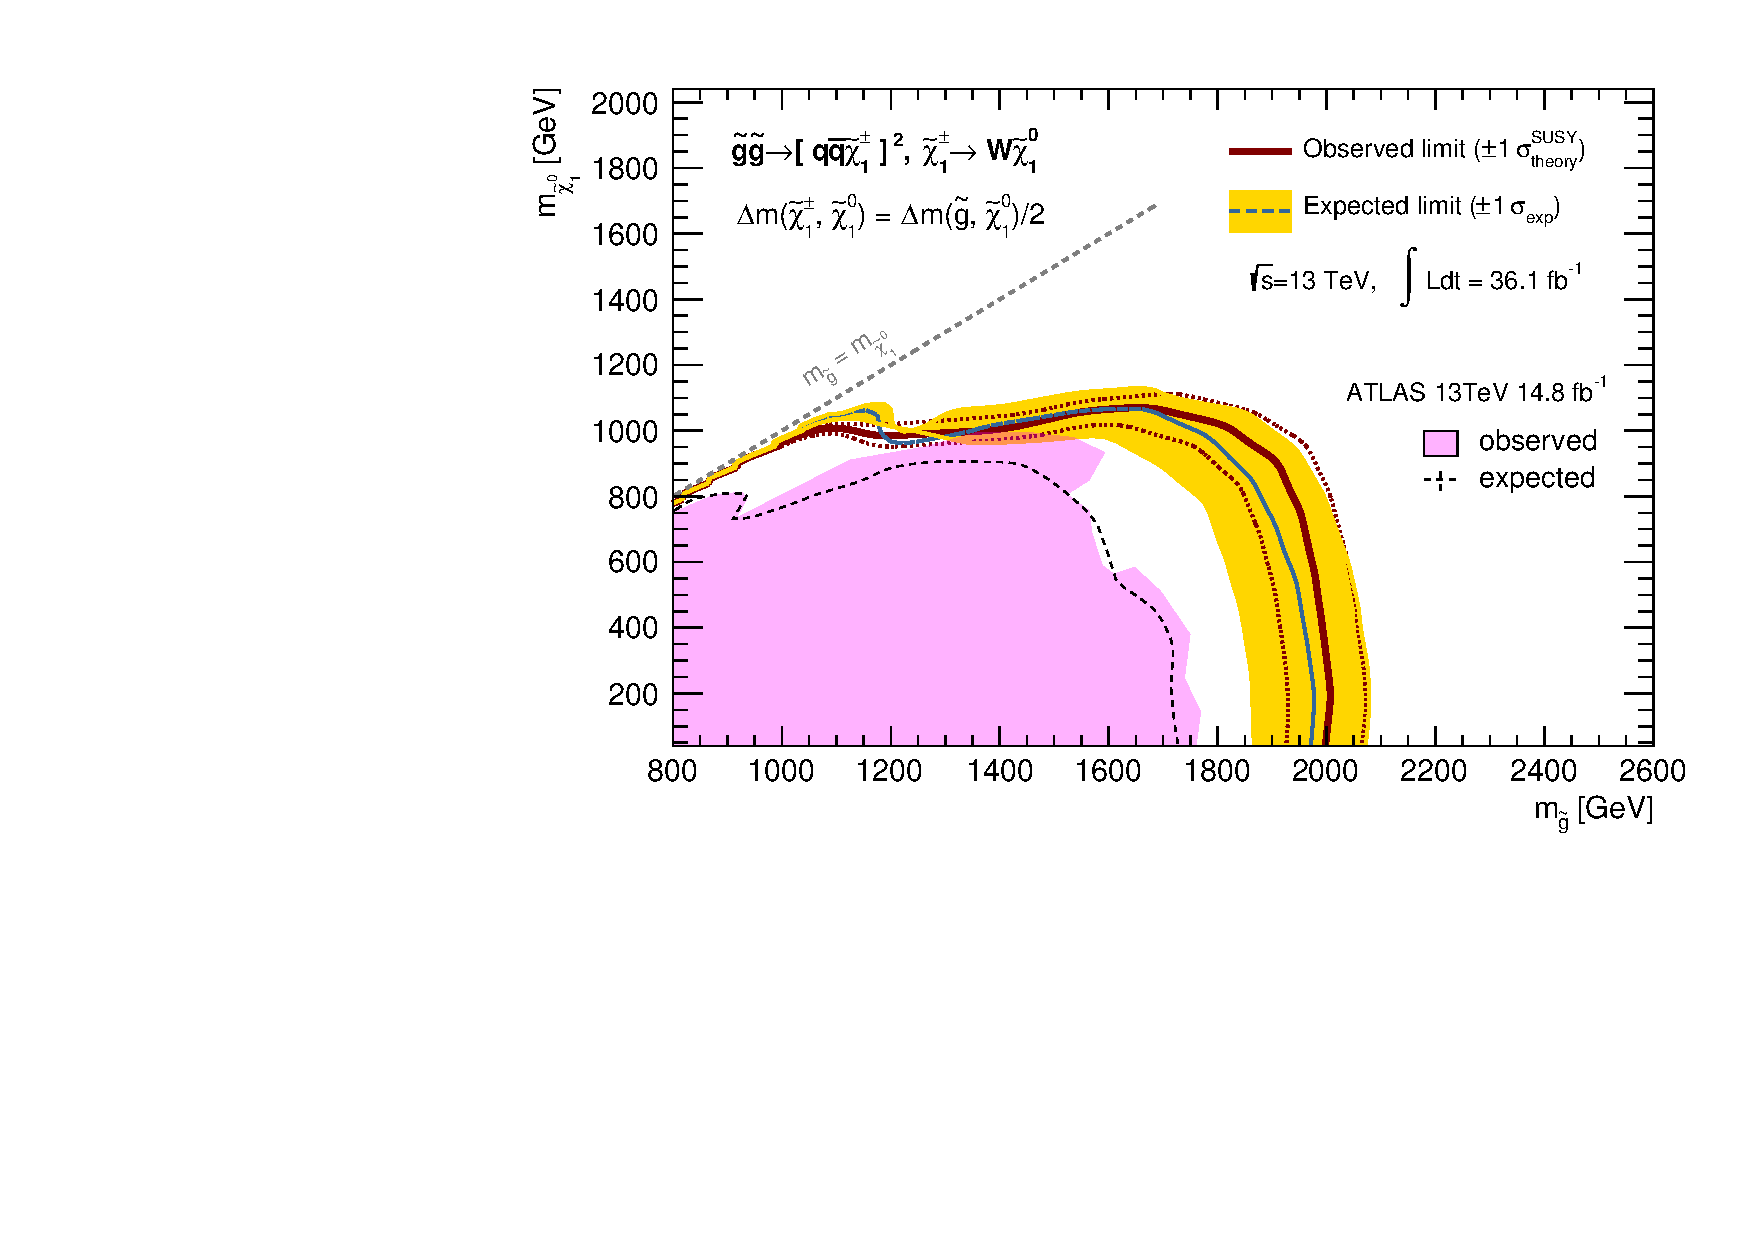
\includegraphics[width=0.48\textwidth]{figures/Result/exclContour/atlascls_wband1_wfixSigXSecband1_showcms0_myAna_tag858_objRep_shapeSys_excl_GG_symQQC1_fixSigXSecNominal_x12_hypotest__1_harvest_list.pdf}}
    \subfigure[]{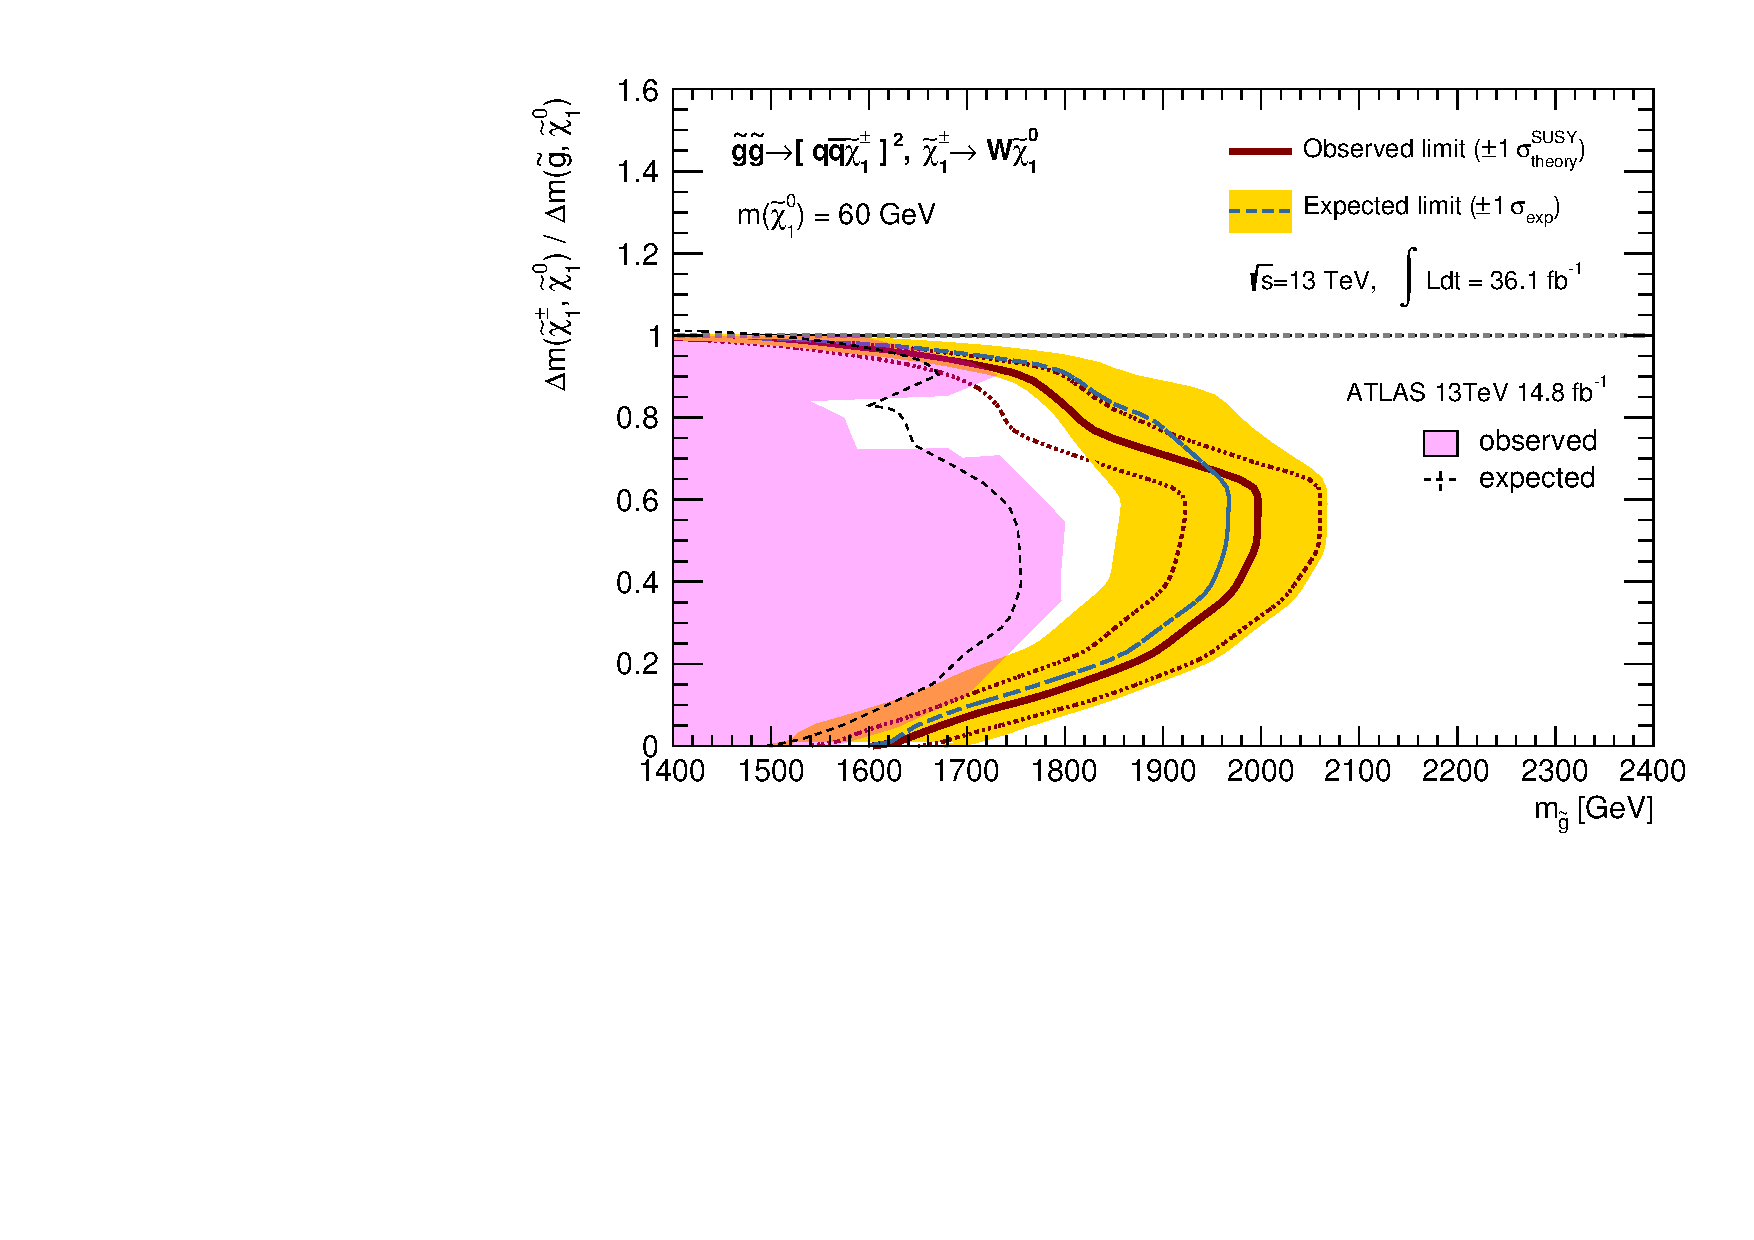
\includegraphics[width=0.48\textwidth]{figures/Result/exclContour/atlascls_wband1_wfixSigXSecband1_showcms0_myAna_tag858_objRep_shapeSys_excl_GG_symQQC1_fixSigXSecNominal_varx_hypotest__1_harvest_list.pdf}}
    \subfigure[]{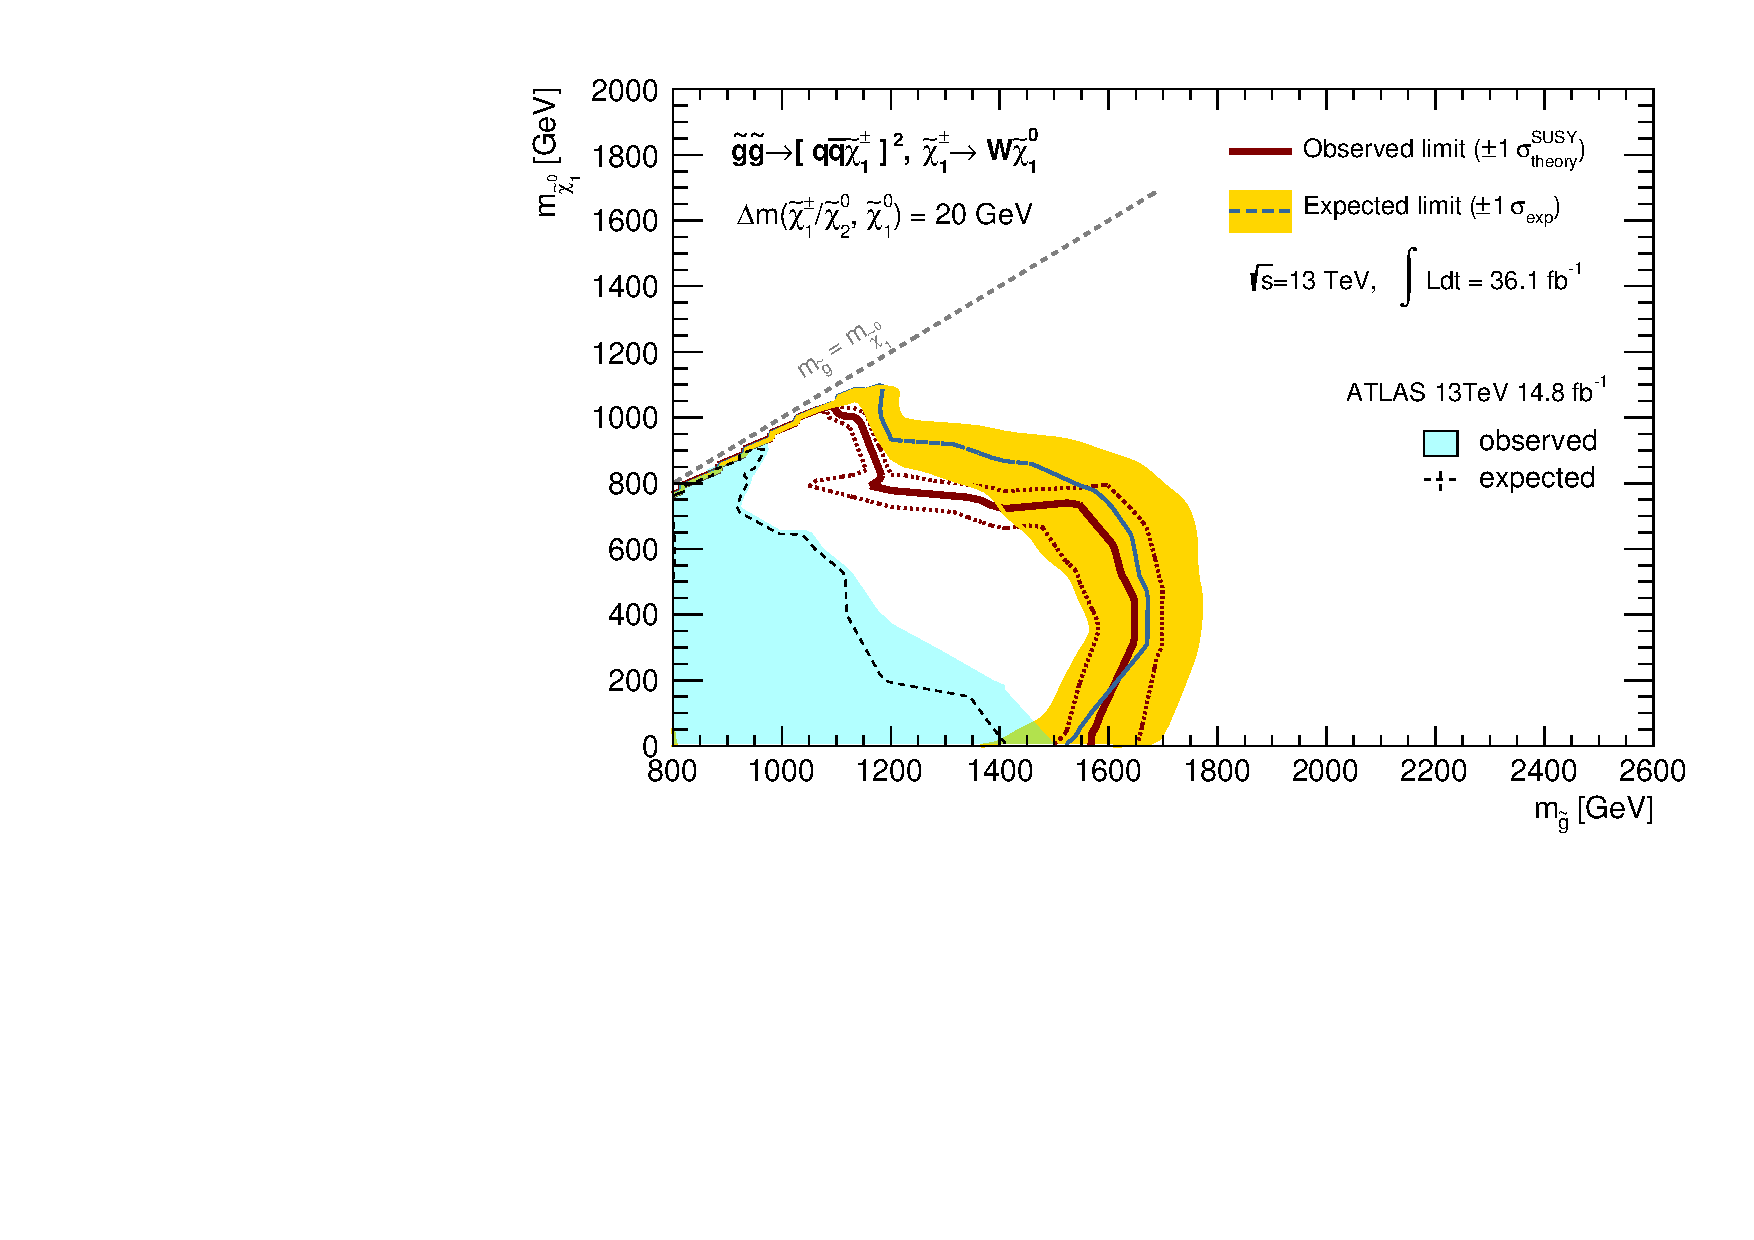
\includegraphics[width=0.48\textwidth]{figures/Result/exclContour/atlascls_wband1_wfixSigXSecband1_showcms0_myAna_tag858_objRep_shapeSys_excl_GG_symQQC1_fixSigXSecNominal_dM20_hypotest__1_harvest_list.pdf}}
    \subfigure[]{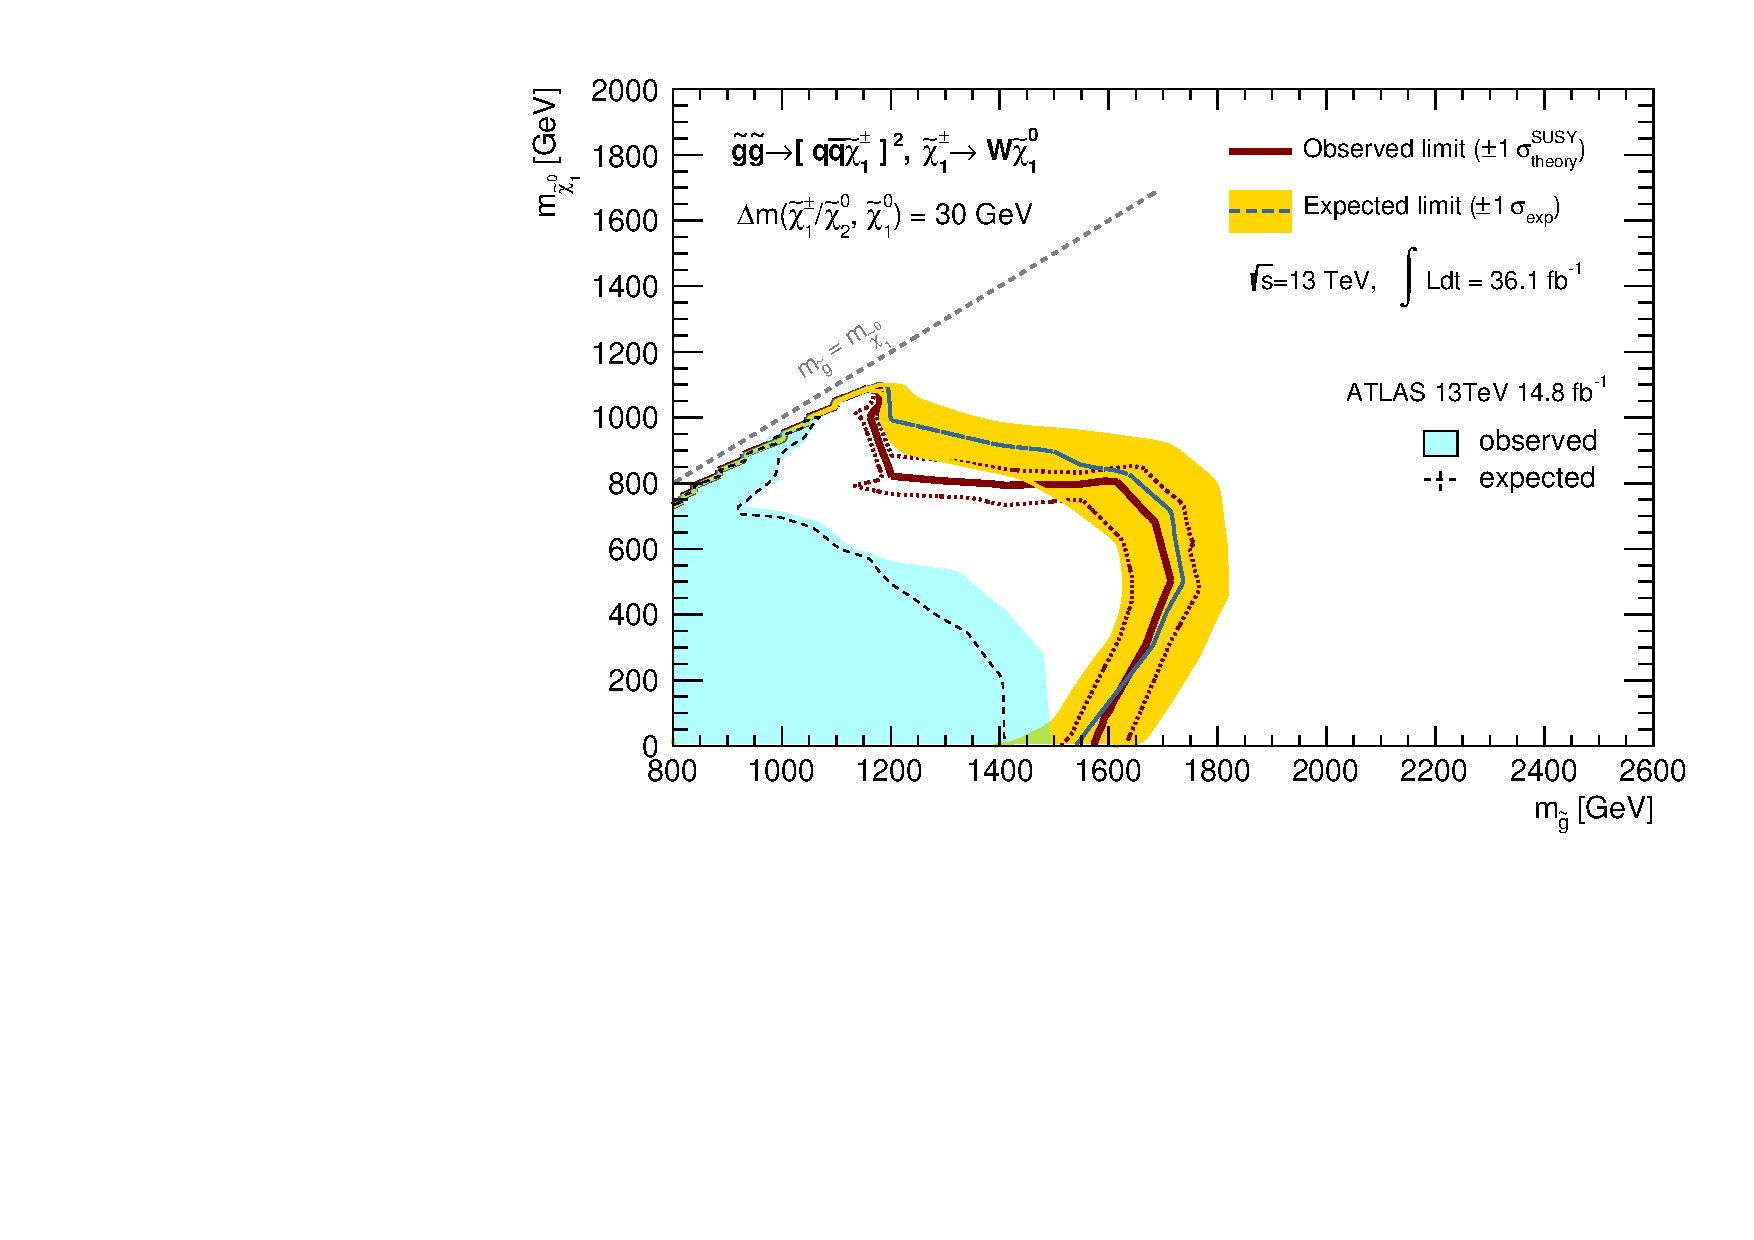
\includegraphics[width=0.48\textwidth]{figures/Result/exclContour/atlascls_wband1_wfixSigXSecband1_showcms0_myAna_tag858_objRep_shapeSys_excl_GG_symQQC1_fixSigXSecNominal_dM30_hypotest__1_harvest_list.pdf}}
    \caption{Exlusion limit for the benchmark model \textbf{QQC1QQC1} presented in the (a) \xhalf (b) \varx (c) \DMtw (d) \DMth grids. Observed limit is shown by the solid red line, while the expected limit are expressed by the dashed blue line with the yellow band describing the variation due to the deviation within $\pm1\sigma$. The up-to-date published result provided by ATLAS \cite{strong1L_ICHEP2016_CONF} is overlaid (observed limit: grey shade, expected limit: black dashed line). All limits correspond to 95$\%$ CL.
  \label{fig::Result::exclLimit::GG_onestepCC} }

\end{figure}


%figures/Result/exclContour/atlascls_wband1_wfixSigXSecband1_showcms0_myAna_tag858_objRep_shapeSys_excl_GG_symQQC1_fixSigXSecNominal_dM20_hypotest__1_harvest_list.pdf

%% --
\begin{figure}[h]
  \centering
    \subfigure[]{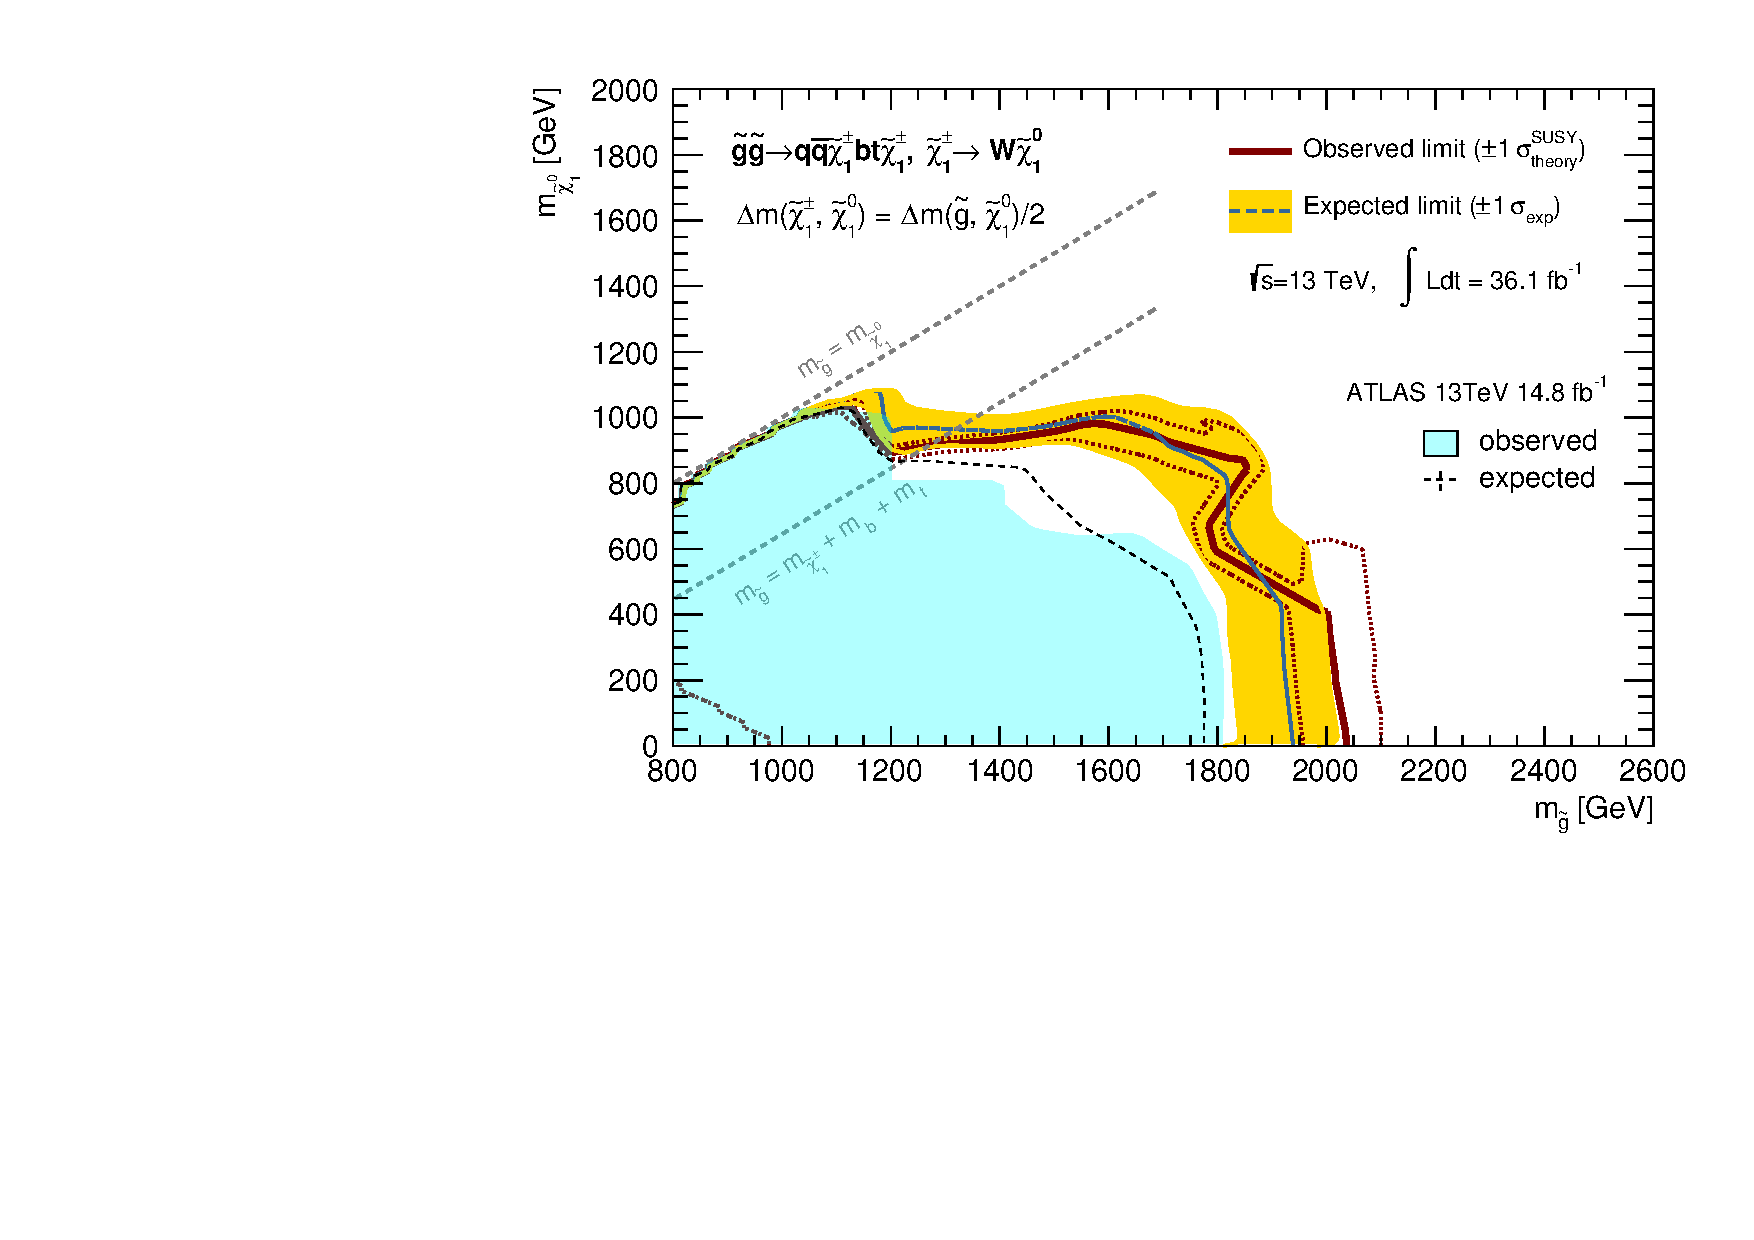
\includegraphics[width=0.48\textwidth]{figures/Result/exclContour/atlascls_wband1_wfixSigXSecband1_showcms0_myAna_tag858_objRep_shapeSys_excl_GG_QQC1BTC1_fixSigXSecNominal_x12_hypotest__1_harvest_list.pdf}}
    \subfigure[]{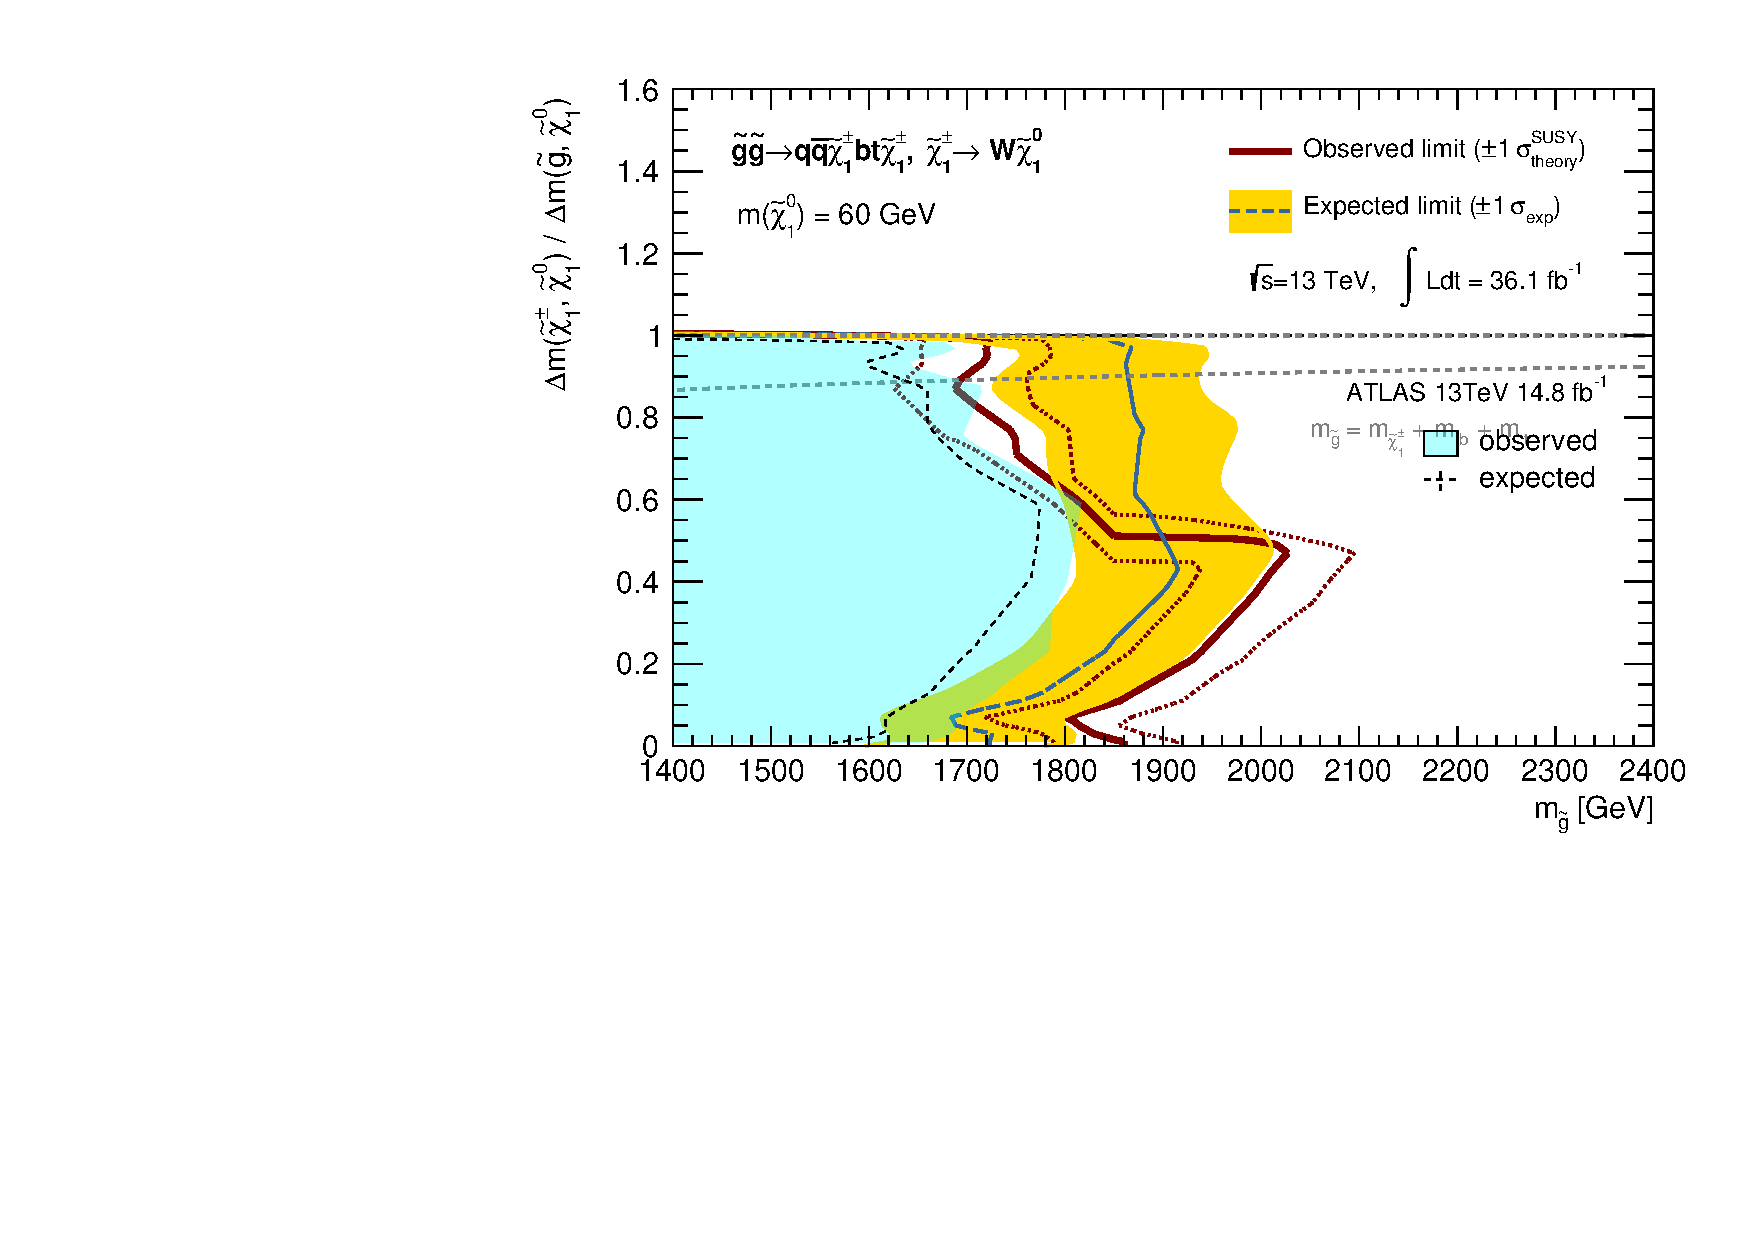
\includegraphics[width=0.48\textwidth]{figures/Result/exclContour/atlascls_wband1_wfixSigXSecband1_showcms0_myAna_tag858_objRep_shapeSys_excl_GG_QQC1BTC1_fixSigXSecNominal_varx_hypotest__1_harvest_list.pdf}}
    \subfigure[]{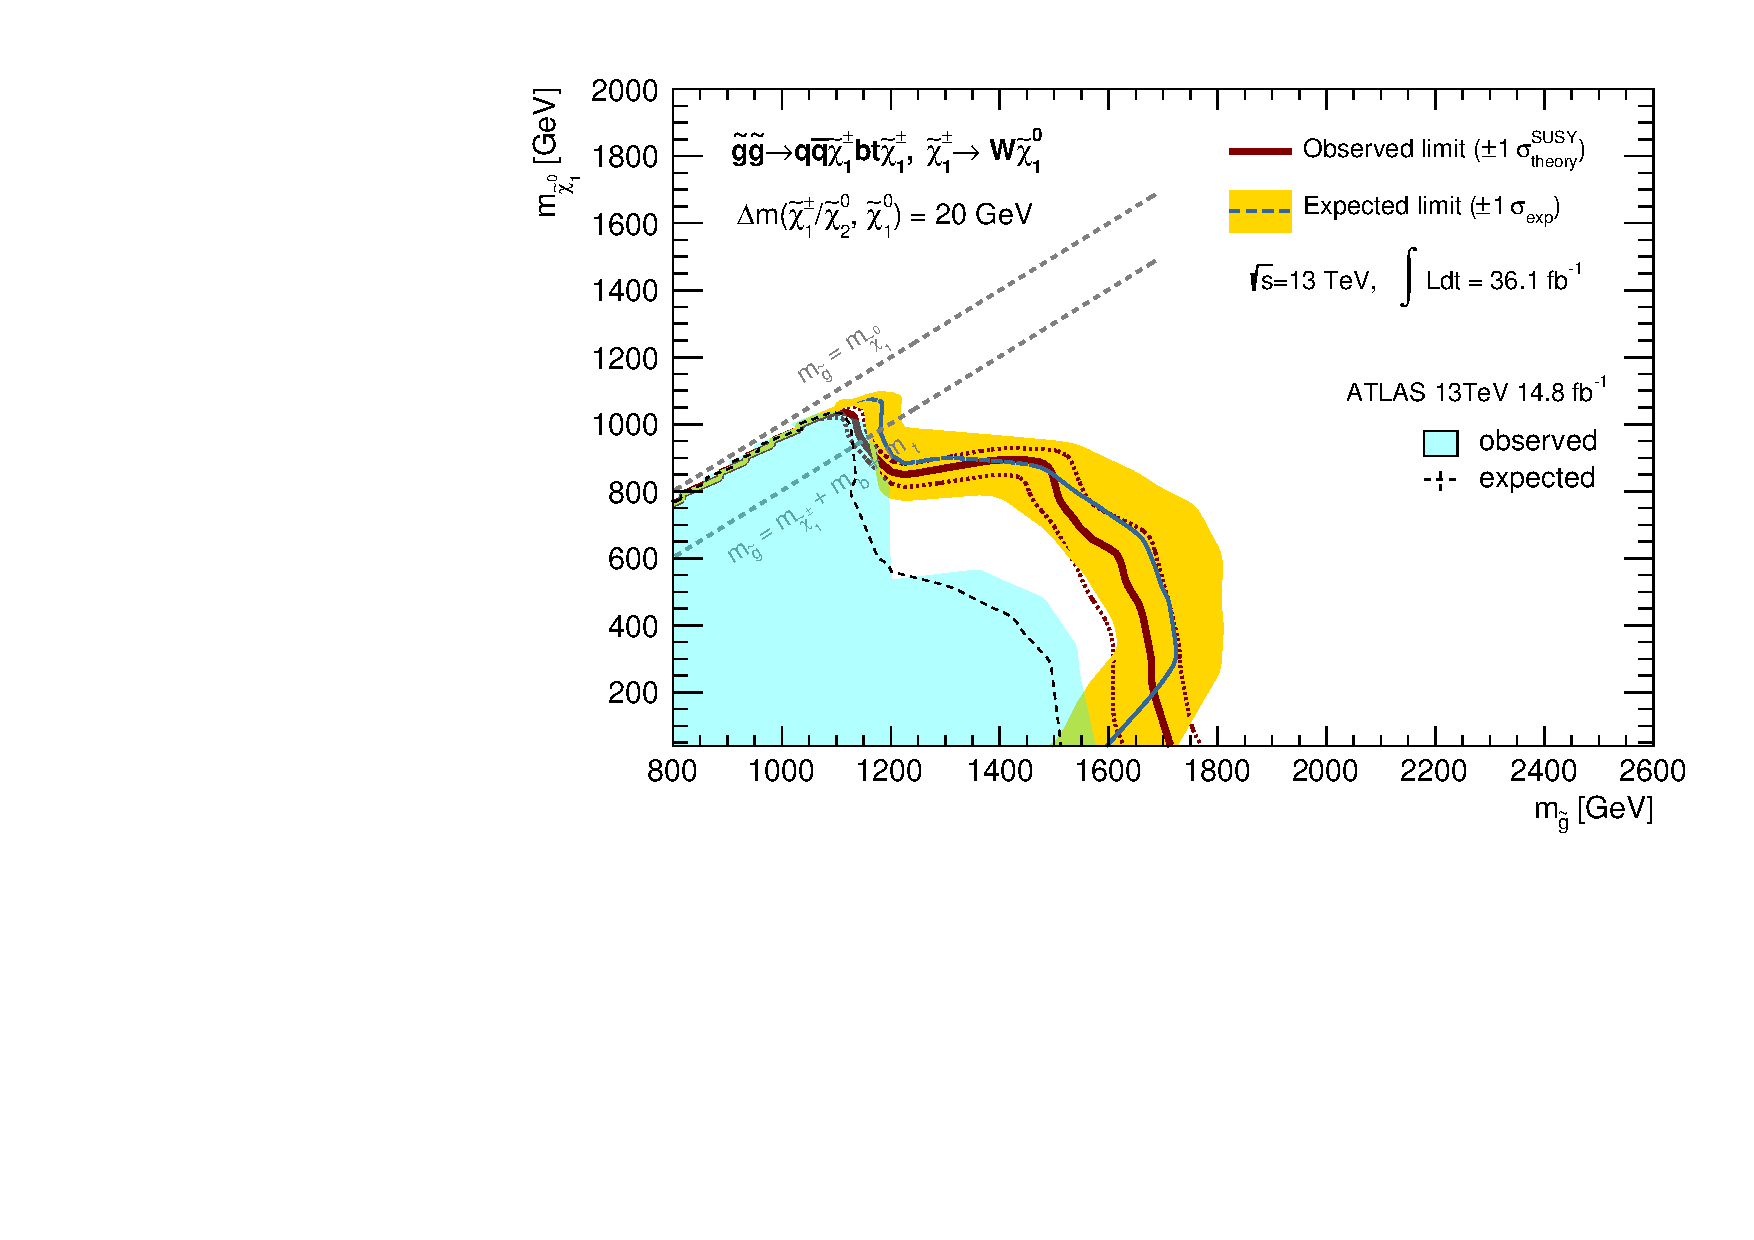
\includegraphics[width=0.48\textwidth]{figures/Result/exclContour/atlascls_wband1_wfixSigXSecband1_showcms0_myAna_tag858_objRep_shapeSys_excl_GG_QQC1BTC1_fixSigXSecNominal_dM20_hypotest__1_harvest_list.pdf}}
    \subfigure[]{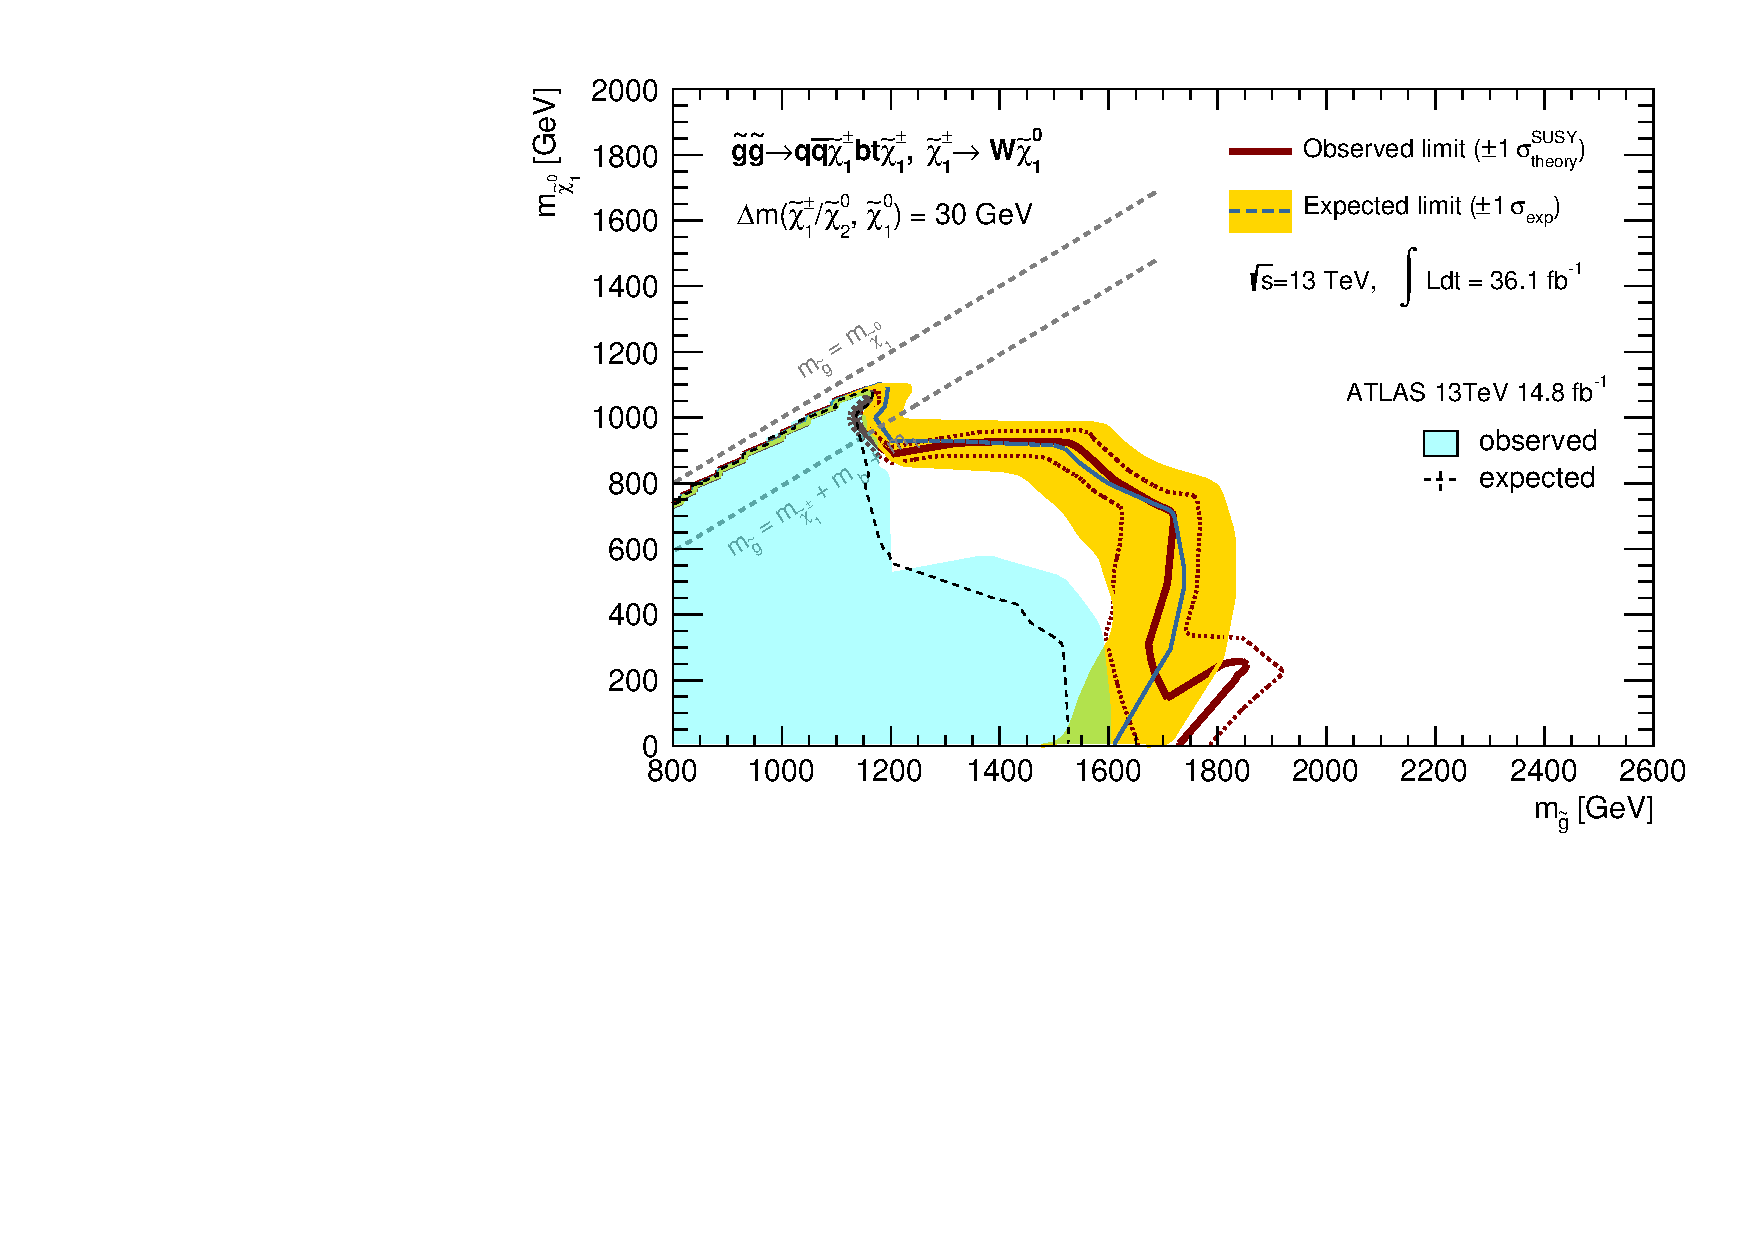
\includegraphics[width=0.48\textwidth]{figures/Result/exclContour/atlascls_wband1_wfixSigXSecband1_showcms0_myAna_tag858_objRep_shapeSys_excl_GG_QQC1BTC1_fixSigXSecNominal_dM30_hypotest__1_harvest_list.pdf}}
    \caption{Projected exlusion limit (95$\%$ CL) for benchmark model \textbf{QQC1BTC1} presented in (a) \xhalf (b) \varx (c) \DMtw (d) \DMth. Observed limit is shown by the solid red line, while the expected limit are expressed by the dashed blue line with the yellow band describing the variation due to the deviation within $\pm1\sigma$. All limits correspond to 95$\%$ CL.
\label{fig::Result::exclLimit::GG_QQC1BTC1} }
\end{figure}

%% --
\begin{figure}
  \begin{center}
    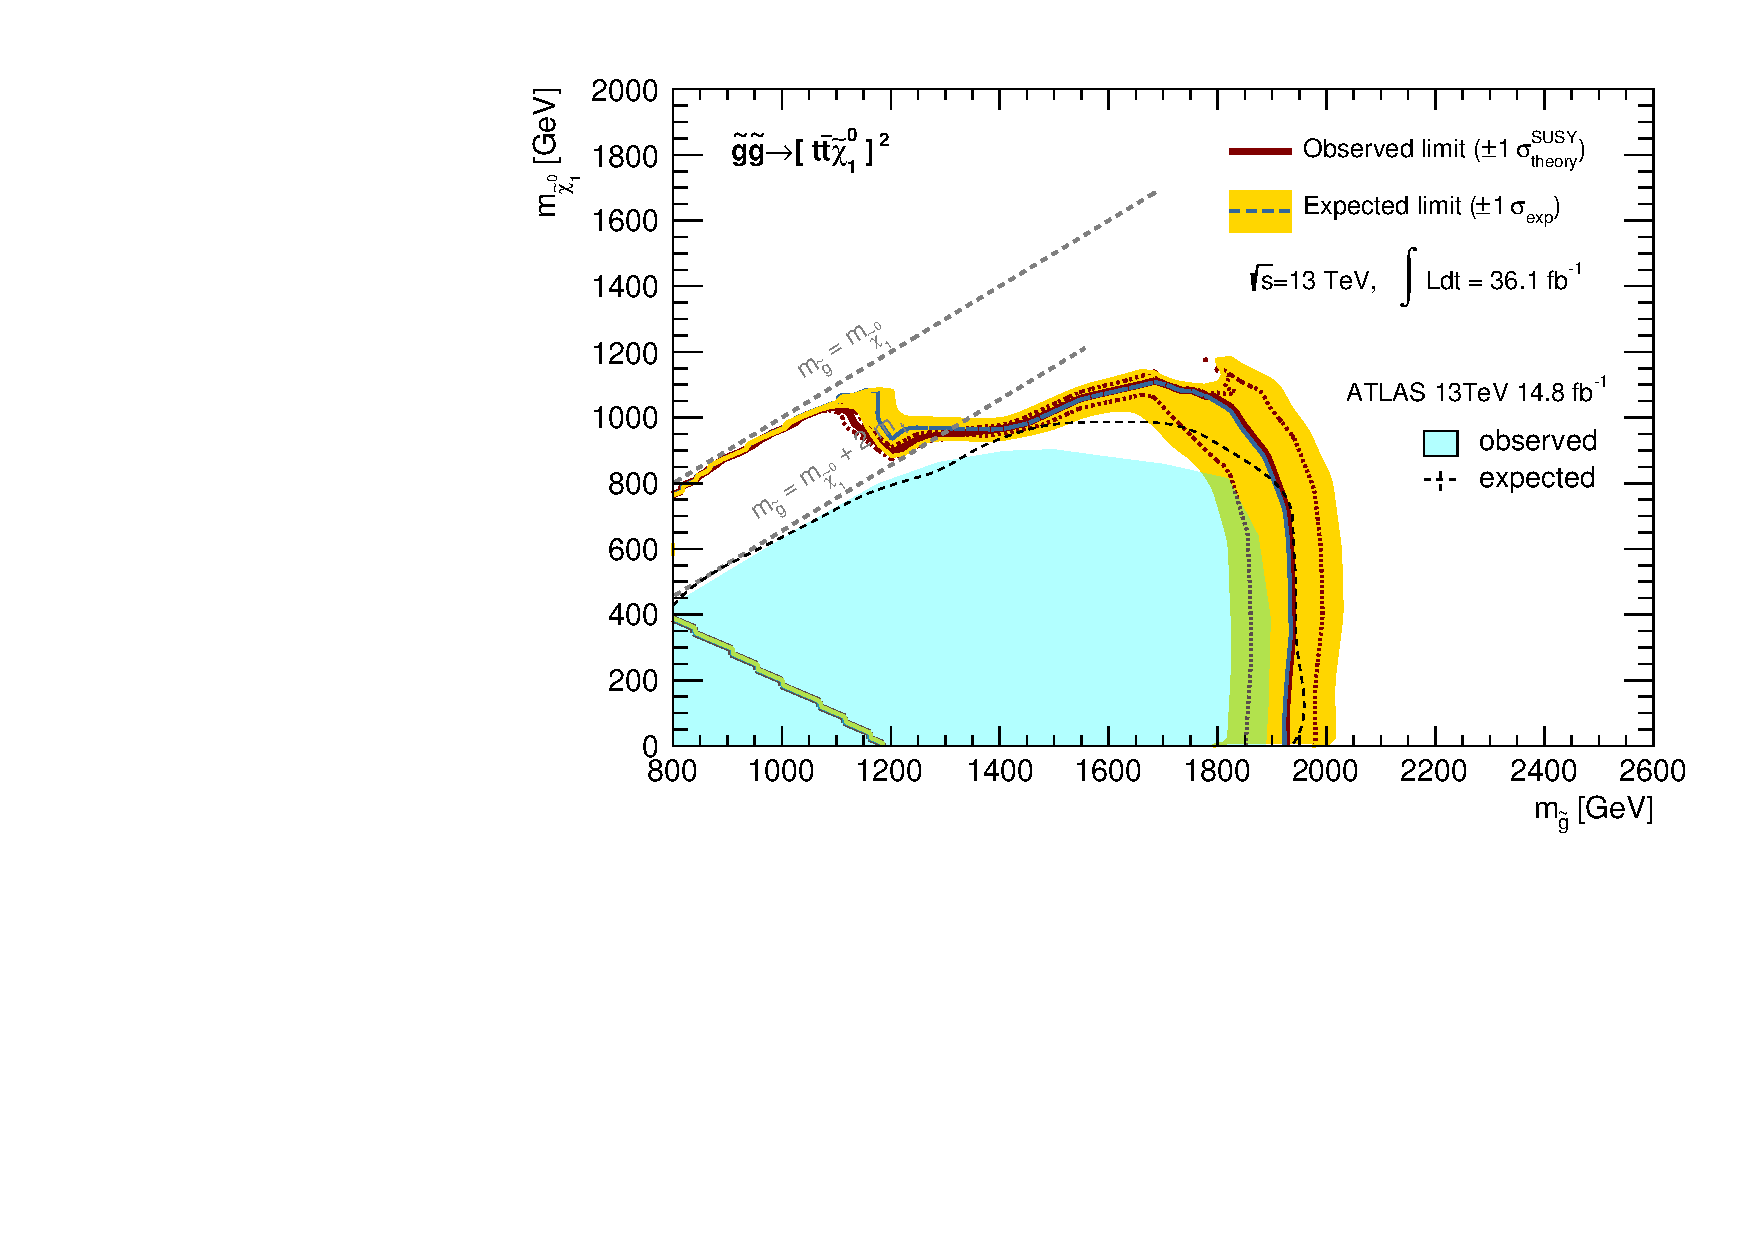
\includegraphics[width=140mm]{figures/Result/exclContour/atlascls_wband1_wfixSigXSecband1_showcms0_myAna_tag858_objRep_shapeSys_excl_GG_symTTN1_fixSigXSecNominal_x12_hypotest__1_harvest_list.pdf}
    \captionof{figure}{Exlusion limit for benchmark model \textbf{TTN1TTN1}.
      Observed limit is shown by the solid red line, while the expected limit are expressed by the dashed blue line with the yellow band describing the variation due to the deviation within $\pm1\sigma$. The up-to-date published result provided by ATLAS \cite{strong3B_ICHEP2016_CONF} is overlaid (observed limit: grey shade, expected limit: black dashed line), which is given by the combination of 0-lepton and 1-lepton analyses. All limits correspond to 95$\%$ CL.
}
    \label{fig::Result::exclLimit::GG_ttn1}
  \end{center}
\end{figure}
%-------------------------------                                                                                                                                                                     



